\section{The Proposed 2s-MDCN}
    \label{mdcn}
    
    \begin{figure}[!htb]
	\centering
	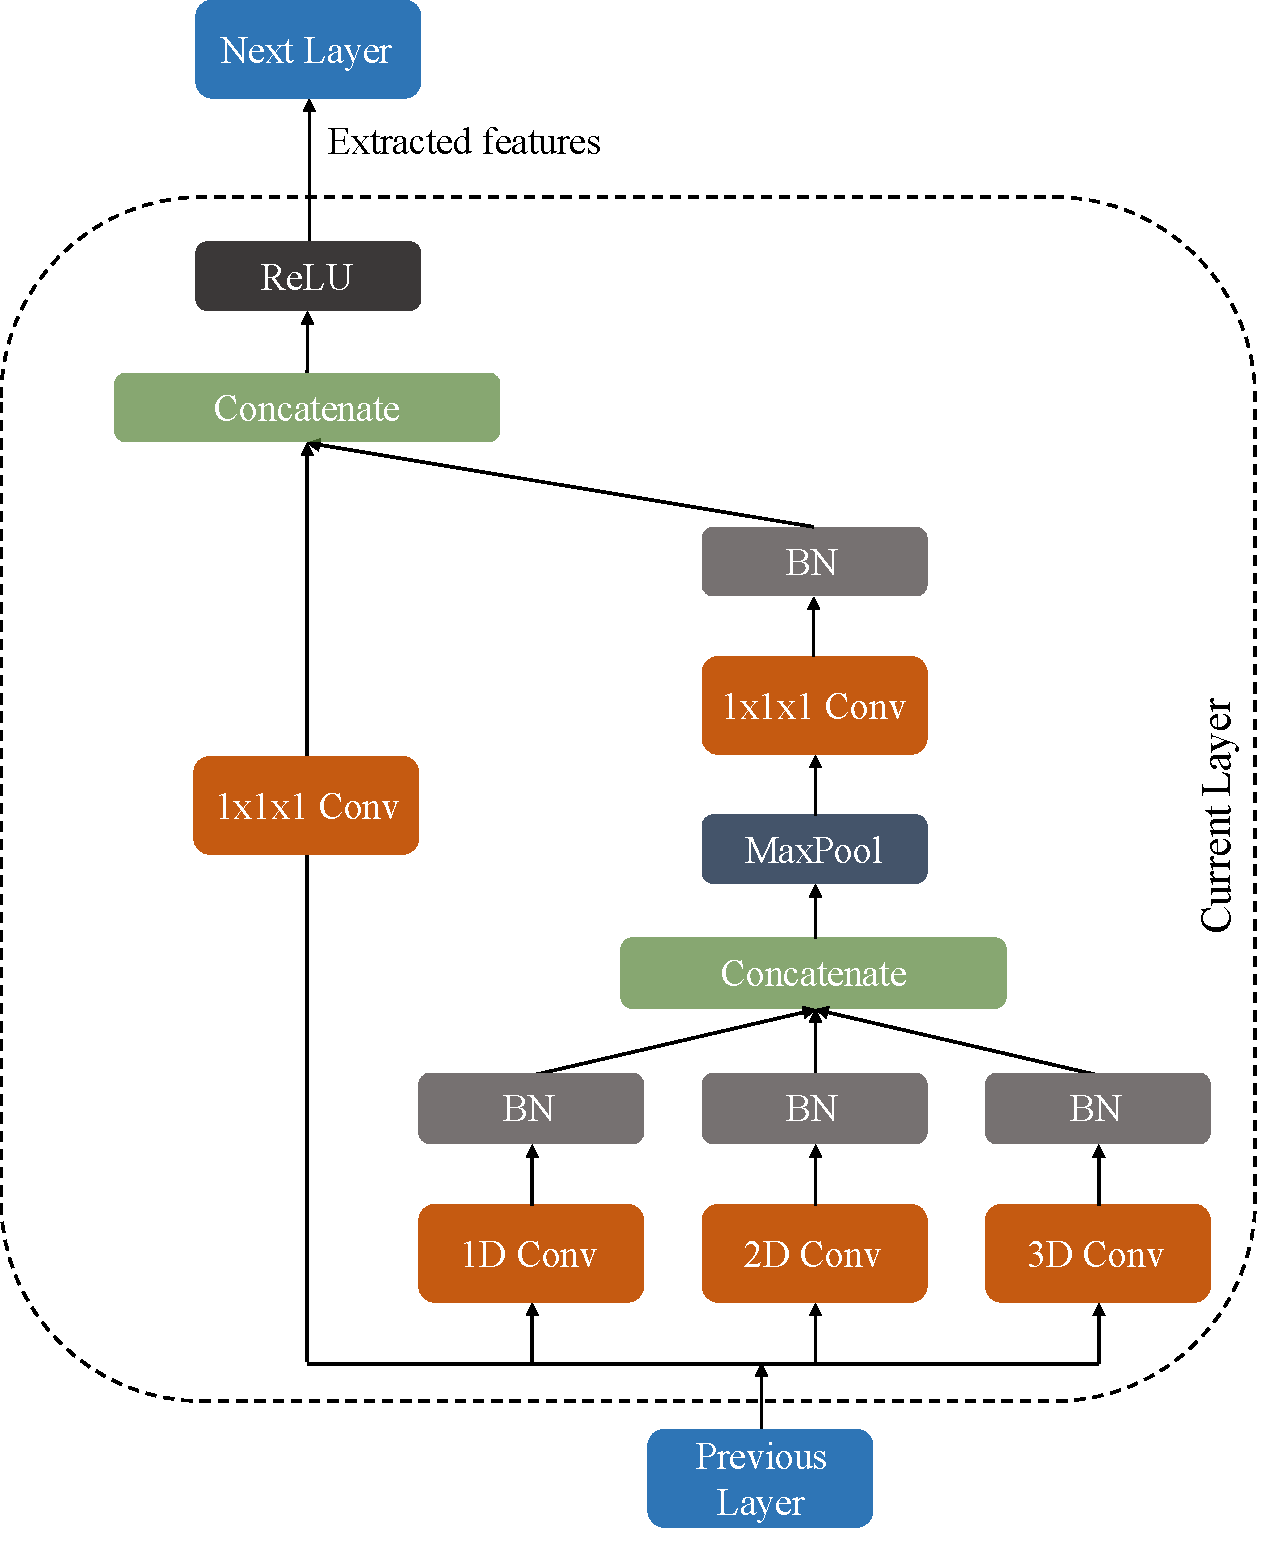
\includegraphics[width=0.9\linewidth]{new_images/mdcn_block.pdf}
	\caption{A single multi-dimensional convolutional block.}
	\label{fig:mdcn_block}
	\end{figure}
    
    In this section, we discuss the architecture of our model in detail. 
    Figure~\ref{fig:pipeline} shows the overall pipeline of our model. 
    Raw RGB frames captured from cameras and optical flow are used as input to the model.
    %add a line here about the first block
    First, the input is passed through a 3D convolutional layer which performs a 3D convolution operation and reduces the size of spatial dimension to prepare for the multi-dimensional convolutional (MDC) blocks.
    Two separate branches are used for RGB frames and optical flow, which are concatenated after the feature extraction from both branches.
%    kernel size  $ {5}\times{7}\times{7} $. 
%    Spatial dimesion was reduced by using a stride of size $ {}\times{}\times{} $
    Each block in the model extracts spatial and temporal features independently from each other and detects violence.
    
    % 	% 	%		%		%		% 	% 	%		%		%		%

%  Block image   %

% 	% 	%		%		%		% 	% 	%		%		%		%		
    
    \subsection{Multi-dimensional Convolutional (MDC) Block}
	The input to each one of the blocks is of shape $ {C}\times{D}\times{H}\times{W} $, where ${C}$ is the number of channels, ${D}$ represents the frame numbers, ${H}$ and ${W}$ denotes height and width respectively. 
	The values in $ {H}\times{W} $ contain spatial information of a particular frame while $ {D} $ frames contain temporal information for the corresponding pixel.
	As figure ~\ref{fig:mdcn_block} illustrates, each block of our proposed model contains three main convolutional layers for extracting spatial and temporal features.
    
    \textbf{ 1D convolutional layer:} The first module is 1D convolutional layer which extracts temporal features from the input.
    The kernel size of this convolutional layer is $ {{k}_{t}}\times{1}\times{1} $. 
    So that it performs convolution operation on a particular pixel over $ {{k}_{t}} $ frames and extracts only temporal information of the corresponding pixel.
    
    \textbf{ 2D convolutional layer:} The second module is 2D convolutional layer which extracts temporal features from the input.
    The kernel size of this convolutional layer is $ {1}\times{{k}_{s}}\times{{k}_{s}} $. 
    So that it performs convolution operation on a single frame and extracts only spatial information from the particular frame.
    
   \textbf{ 3D convolutional layer:} The second module is 3D convolutional layer which extracts both spatial and temporal features from the input.
    The kernel size of this convolutional layer is $ {{k}_{t}}\times{{k}_{s}}\times{{k}_{s}} $. 
    So that it performs convolution operation over ${{k}_{t}}$ frames and extracts temporal and spatial frames together.
    
    Each of these three modules is followed by a batch normalization layer.
    In our model, we used $ 3 $ the value of $ {{k}_{t}} $ and $ {{k}_{s}} $.
    They extract information independently from the same spatio-teporal position of  the input and fuse together.
    In this process, our model can extract all the information from the input which reduces information loss and improves accuracy.
    Then, the 
%    three modules are followed by a 
	fused features are passed through a 
    $maxpooling$ layer and a $ {1}\times{1}\times{1} $ convolution layer which reduces the number of channels for the next layer.
    This reduction module keeps our model size small.
    Moreover, a concatenated skip connection~\cite{huang2017densely}, followed by a ReLU layer, is added to stabilize the model which also helped to improve accuracy.
    Skip connection concatenates features from the previous layers to the current layer which allows more information to be obtained from the previous layers and reduces loss of information. Concatenated skip connections also help the gradient to propagate better and fix the vanishing gradient problem.
    To match the input channel to the output channel, we have used a convolutional layer of kernel size ${1}\times{1}\times{1}$ and stride of size ${1}\times{2}\times{2}$.

	% 	% 	%		%		%		% 	% 	%		%		%		%

%  Full-network image   %

% 	% 	%		%		%		% 	% 	%		%		%		%		
	
	
	\begin{figure}[!htb]
	\centering
	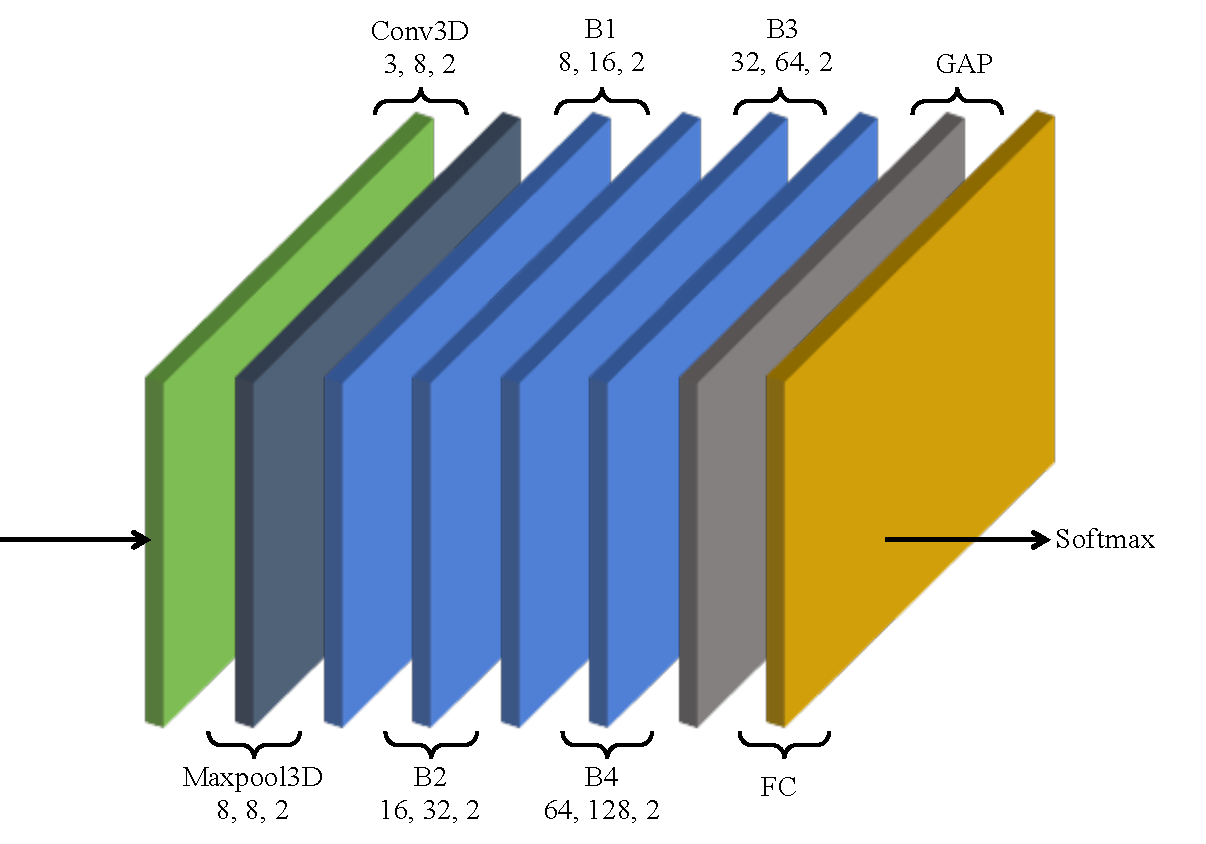
\includegraphics[width=0.9\linewidth]{new_images/vio_fullnet_pdf.pdf}
	\caption{Layers of 2s-MDCN.}
	\label{fig:full_network}
	\end{figure}      
    
    % Please add the following required packages to your document preamble:
% \usepackage{multirow}
\begin{table*}[]
\centering
\begin{tabular}{|cc|cc|cc|}
\hline
\multicolumn{2}{|c|}{\multirow{2}{*}{Layers}}                                                   & \multicolumn{2}{c|}{2s-MDCN}               & \multicolumn{2}{c|}{\multirow{2}{*}{Output Size}} \\ \cline{3-4}
\multicolumn{2}{|c|}{}                                                                          & \multicolumn{1}{c|}{RGB} & optical flow & \multicolumn{2}{c|}{}                             \\ \hline
\multicolumn{2}{|c|}{\multirow{2}{*}{input}}                                                    & \multicolumn{2}{c|}{\multirow{2}{*}{}}  & \multicolumn{2}{c|}{$3\times32\times{224}^2$(RGB)}       \\ 
\multicolumn{2}{|c|}{}  & \multicolumn{2}{c|}{} & \multicolumn{2}{c|}{$2\times32\times{224}^2$(optical flow)}               \\ \hline
\multicolumn{2}{|c|}{conv$_1$}  & \multicolumn{2}{c|}{conv 3D: ${5}\times{{7}^2} $, stride:  ${1}\times{{2}^2} $}               & \multicolumn{2}{c|}{$8\times{32}\times{112}^2$} \\ \hline

\multicolumn{2}{|c|}{pool$_1$}  & \multicolumn{2}{c|}{max pool: ${1}\times{{3}^2}$, stride:  ${1}\times{{2}^2} $}               & \multicolumn{2}{c|}{$8\times{32}\times{56}^2$} \\ \hline

\multicolumn{1}{|c|}{\multirow{4}{*}{mdcn$_1$}} & \multicolumn{1}{c|}{\multirow{3}{*}{conv layer}} & \multicolumn{2}{c|}{conv 1D: ${3}\times{{1}^2}$}   & \multicolumn{2}{c|}{\multirow{4}{*}{$16\times{32}\times{28}^2$}}      \\
\multicolumn{1}{|c|}{}                       & \multicolumn{1}{c|}{}                            & \multicolumn{2}{c|}{conv 2D: ${1}\times{{3}^2} $}           & \multicolumn{2}{c|}{}                             \\
\multicolumn{1}{|c|}{}                       & \multicolumn{1}{c|}{}                            & \multicolumn{2}{c|}{conv 3D: ${3}\times{{3}^2} $}           & \multicolumn{2}{c|}{}                             \\ \cline{2-4}

\multicolumn{1}{|c|}{}                                     & \multirow{2}{*}{fuse and reduce} & \multicolumn{2}{c|}{max pool: ${1}\times{{3}^2} $, stride:  ${1}\times{{2}^2} $ }            & \multicolumn{2}{c|}{}     \\
\multicolumn{1}{|c|}{}   &       & \multicolumn{2}{c|}{conv: ${1}\times{{1}^2} $ }  & \multicolumn{2}{c|}{} \\ \hline


\multicolumn{1}{|c|}{\multirow{4}{*}{mdcn$_2$}} & \multicolumn{1}{c|}{\multirow{3}{*}{conv layer}} & \multicolumn{2}{c|}{conv 1D: ${3}\times{{1}^2}$}   & \multicolumn{2}{c|}{\multirow{4}{*}{$32\times{32}\times{28}^2$}}      \\
\multicolumn{1}{|c|}{}                       & \multicolumn{1}{c|}{}                            & \multicolumn{2}{c|}{conv 2D: ${1}\times{{3}^2} $}           & \multicolumn{2}{c|}{}                             \\
\multicolumn{1}{|c|}{}                       & \multicolumn{1}{c|}{}                            & \multicolumn{2}{c|}{conv 3D: ${3}\times{{3}^2} $}           & \multicolumn{2}{c|}{}                             \\ \cline{2-4}

\multicolumn{1}{|c|}{}                                     & \multirow{2}{*}{fuse and reduce} & \multicolumn{2}{c|}{max pool: ${1}\times{{3}^2} $, stride:  ${1}\times{{2}^2} $ }            & \multicolumn{2}{c|}{}     \\ 
\multicolumn{1}{|c|}{}   &       & \multicolumn{2}{c|}{conv: ${1}\times{{1}^2} $ }  & \multicolumn{2}{c|}{} \\ \hline


\multicolumn{1}{|c|}{\multirow{4}{*}{mdcn$_3$}} & \multicolumn{1}{c|}{\multirow{3}{*}{conv layer}} & \multicolumn{2}{c|}{conv 1D: ${3}\times{{1}^2}$}   & \multicolumn{2}{c|}{\multirow{4}{*}{$64\times{32}\times{14}^2$}}      \\
\multicolumn{1}{|c|}{}                       & \multicolumn{1}{c|}{}                            & \multicolumn{2}{c|}{conv 2D: ${1}\times{{3}^2} $}           & \multicolumn{2}{c|}{}                             \\
\multicolumn{1}{|c|}{}                       & \multicolumn{1}{c|}{}                            & \multicolumn{2}{c|}{conv 3D: ${3}\times{{3}^2} $}           & \multicolumn{2}{c|}{}                             \\ \cline{2-4}

\multicolumn{1}{|c|}{}                                     & \multirow{2}{*}{fuse and reduce} & \multicolumn{2}{c|}{max pool: ${1}\times{{3}^2} $, stride:  ${1}\times{{2}^2} $ }            & \multicolumn{2}{c|}{}     \\ 
\multicolumn{1}{|c|}{}   &       & \multicolumn{2}{c|}{conv: ${1}\times{{1}^2} $ }  & \multicolumn{2}{c|}{} \\ \hline


\multicolumn{1}{|c|}{\multirow{4}{*}{mdcn$_4$}} & \multicolumn{1}{c|}{\multirow{3}{*}{conv layer}} & \multicolumn{2}{c|}{conv 1D: ${3}\times{{1}^2}$}   & \multicolumn{2}{c|}{\multirow{4}{*}{$128\times{32}\times{7}^2$}}      \\
\multicolumn{1}{|c|}{}                       & \multicolumn{1}{c|}{}                            & \multicolumn{2}{c|}{conv 2D: ${1}\times{{3}^2} $}           & \multicolumn{2}{c|}{}                             \\
\multicolumn{1}{|c|}{}                       & \multicolumn{1}{c|}{}                            & \multicolumn{2}{c|}{conv 3D: ${3}\times{{3}^2} $}           & \multicolumn{2}{c|}{}                             \\ \cline{2-4}

\multicolumn{1}{|c|}{}                                     & \multirow{2}{*}{fuse and reduce} & \multicolumn{2}{c|}{max pool: ${1}\times{{3}^2} $, stride:  ${1}\times{{2}^2} $ }            & \multicolumn{2}{c|}{}     \\ 
\multicolumn{1}{|c|}{}   &       & \multicolumn{2}{c|}{conv: ${1}\times{{1}^2} $ }  & \multicolumn{2}{c|}{} \\ \hline

\multicolumn{4}{|c|}{concatenate, global average pool, fc}                                                                                & \multicolumn{2}{c|}{\#classes (2)}                \\ \hline
\end{tabular}
\caption{ Overall architecture of 2s-MDCN.}

    \label{tab:network_table}
\end{table*}





% \begin{table*}[t]
% \begin{center}
% \begin{tabular}{c|c|c|c}
% \hline
% \multicolumn{2}{c|}{Layers}                & \multicolumn{1}{c|}{MDCN} & \multicolumn{1}{c}{Output Size}                  \\ \hline
% \multicolumn{2}{c|}{input layer}           &                           & $3\times{32}\times{224}^2$                                       \\ \hline
% \multicolumn{2}{c|}{\multirow{1}{*}{conv$_1$}} &conv: ${5}\times{{7}^2} $, stride:  ${1}\times{{2}^2} $        & \multicolumn{1}{c}{\multirow{1}{*}{$8\times{32}\times{112}^2$}} \\
% %\multicolumn{2}{c|}{}                      &                    & \multicolumn{1}{c}{}                             \\ \hline
% \hline
% \multicolumn{2}{c|}{\multirow{1}{*}{pool$_1$}} & max pool: ${1}\times{{3}^2}$, stride:  ${1}\times{{2}^2} $         & \multicolumn{1}{c}{\multirow{1}{*}{$8\times{32}\times{56}^2$}} \\
% %\multicolumn{2}{c|}{}                      & stride                    & \multicolumn{1}{c}{}                             \\ \hline
% \hline

% \multicolumn{1}{l|}{\multirow{5}{*}{mdcn$_1$}} & \multirow{3}{*}{conv layers} & conv: ${3}\times{{1}^2} $       & \multirow{5}{*}{$16\times{32}\times{28}^2$}               \\
% \multicolumn{1}{l|}{}                       &                                        & conv: ${1}\times{{3}^2} $                     &                                                   \\
% \multicolumn{1}{l|}{}                       &                                        & conv: ${3}\times{{3}^2} $                     &                                                   \\ \cline{2-3}
% \multicolumn{1}{l|}{}                       & \multirow{2}{*}{fuse and reduce}       & max pool: ${1}\times{{3}^2} $, stride:  ${1}\times{{2}^2} $        &                                                   \\
% \multicolumn{1}{l|}{}                       &                                        & conv: ${1}\times{{1}^2} $                &        \\
% \hline

% \multicolumn{1}{l|}{\multirow{5}{*}{mdcn$_2$}} & \multirow{3}{*}{conv layers} & conv: ${3}\times{{1}^2} $       & \multirow{5}{*}{$32\times{32}\times{28}^2$}             \\
% \multicolumn{1}{l|}{}                       &                                        & conv: ${1}\times{{3}^2} $                     &                                                   \\
% \multicolumn{1}{l|}{}                       &                                        & conv: ${3}\times{{3}^2} $                       &                                                   \\ \cline{2-3}
% \multicolumn{1}{l|}{}                       & \multirow{2}{*}{fuse and reduce}       & max pool: ${1}\times{{3}^2} $, stride:  ${1}\times{{2}^2} $                       &                                                   \\
% \multicolumn{1}{l|}{}                       &                                        & conv: ${1}\times{{1}^2} $                 &        \\
% \hline

% \multicolumn{1}{l|}{\multirow{5}{*}{mdcn$_3$}} & \multirow{3}{*}{conv layers} & conv: ${3}\times{{1}^2} $              & \multirow{5}{*}{$64\times{32}\times{14}^2$}          \\
% \multicolumn{1}{l|}{}                       &                                        & conv: ${1}\times{{3}^2} $                       &                                                   \\
% \multicolumn{1}{l|}{}                       &                                        & conv: ${3}\times{{3}^2} $                    &                                                   \\ \cline{2-3}
% \multicolumn{1}{l|}{}                       & \multirow{2}{*}{fuse and reduce}       & max pool: ${1}\times{{3}^2} $, stride:  ${1}\times{{2}^2} $                      &                                                   \\
% \multicolumn{1}{l|}{}                       &                                        & conv: ${1}\times{{1}^2} $                 &        \\
% \hline

% \multicolumn{1}{l|}{\multirow{5}{*}{mdcn$_4$}} & \multirow{3}{*}{conv layers} & conv: ${3}\times{{1}^2} $          & \multirow{5}{*}{$128\times{32}\times{7}^2$}                \\
% \multicolumn{1}{l|}{}                       &                                        & conv: ${1}\times{{3}^2} $                     &                                                   \\
% \multicolumn{1}{l|}{}                       &                                        & conv: ${3}\times{{3}^2} $                      &                                                   \\ \cline{2-3}
% \multicolumn{1}{l|}{}                       & \multirow{2}{*}{fuse and reduce}       & max pool: ${1}\times{{3}^2} $, stride:  ${1}\times{{2}^2} $                      &                                                   \\
% \multicolumn{1}{l|}{}                       &                                        & conv: ${1}\times{{1}^2} $                 &        \\
% \hline

% \multicolumn{3}{c|}{global average pool, fc}                                                                     & {\#classes ($2$)}\\
% \hline
% \end{tabular}
% \end{center}
% \caption{ Multi-dimensional convolutional architecture for violence detection.}

%     \label{tab:network_table}
% \end{table*}









    
    \subsection{Multi-dimensional Convolutional Network}
   As figure ~\ref{fig:full_network} illustrates, our proposed network consists of $ 4 $ MDC blocks and a 3D convolutional layer at the beginning. 
   Both RGB and optical flow streams have identical numbers of MDC blocks.
   The first 3D convolutional layer is of kernel size $ {5}\times{7}\times{7} $ and stride of size $ {1}\times{2}\times{2} $.
   This layer is followed by a $ maxpool $ layer with stride value of $ {1}\times{2}\times{2} $.
   The convolution layer and $maxpool$ layer are used to reduce the size of spatial dimension.
   The output from these layers is passed into the $ 4 $ MDC blocks, where temporal and spatial information are extracted.
   The numbers of channels of output from the convolution blocks are $8$, $16$, $32$, $64$, and $128$.
   After extracting features from RGB and optical flow stream, they are concatenated and a $global$ $average$ $pooling$ layer is used to combine and reduce the extracted feature and finally, a fully connected (FC) and $softmax$ layer is used to detect violence.
   Table~\ref{tab:network_table} displays the kernel size, stride size, and number output channel of each block in detail.
   The shape of convolutional kernel is denoted by $ {T}\times{S}^2 $, where $T$ kernel temporal dimension and $S$ indicated spatial dimension. Stride is also represented in the same manner (temporal stride, spatial stride$^2$). The output size is represented by channel$\times$temporal length$\times$spatial dimension$^2$. The features are passed into $conv$ $layers$ independently and then concatenated and passed into $fuse$ $and$ $reduce$ layer.
   
   
   	
	
 